\documentclass{article}

\usepackage{lipsum}
\usepackage[margin=1in,includefoot]{geometry}
\usepackage{graphicx}
\usepackage{float}
\usepackage[hidelinks]{hyperref}
\usepackage{amsmath}
\usepackage{amssymb}
\usepackage{color}

\usepackage[usenames,dvipsnames]{xcolor}
\usepackage{listings}


% Header and Footer Stuff
\usepackage{fancyhdr}
\pagestyle{fancy}
\fancyhead{}
\fancyfoot{}
\fancyfoot[R]{\thepage}
\renewcommand{\headrulewidth}{0pt}
\renewcommand{\footrulewidth}{0pt}


\definecolor{dkgreen}{rgb}{0,0.6,0}
\definecolor{gray}{rgb}{0.5,0.5,0.5}
\definecolor{mauve}{rgb}{0.58,0,0.82}

\lstset{
  language=VHDL,
  aboveskip=3mm,
  belowskip=3mm,
  showstringspaces=false,
  columns=flexible,
  basicstyle={\small\ttfamily},
  numbers=none,
  numberstyle=\tiny\color{gray},
  keywordstyle=\color{blue},
  commentstyle=\color{dkgreen},
  stringstyle=\color{mauve},
  breaklines=true,
  breakatwhitespace=true,
  tabsize=3
}


\begin{document}

\begin{titlepage}
	\begin{center}
	\begin{align*}
	
\includegraphics[height=1.75in]{logo.png}
	\end{align*}


	
	\line(1,0){300}\\
	[0.25in]
	\huge{\bfseries Tutorial 2 }\\
	[2mm]
	\line(1,0){200}\\
	[1.5cm]
	\textsc{\LARGE Transformations}\\
	[0.75cm]
	\textsc{\Large CS4052 Computer Graphics}\\
	[7cm]	
	\end{center}
	
	
	
	\begin{flushright}
	\textsc{\large Alexandru Sulea\\
	D Stream\\
	\#12315152\\
	18 Octomber 2016\\}
	\end{flushright}
	
\end{titlepage}
%Table of Contents Stuff%
%\tableofcontents
%\listoffigures
%\addcontentsline{toc}{section}{List of Figures}
%\listoftables
%\addcontentsline{toc}{section}{List of Tables}


\thispagestyle{empty}
\cleardoublepage
\pagenumbering{arabic}
\setcounter{page}{1}

\pagebreak
\section{Overview}
I used the math file provided for the identity, translation, rotation and scaling matrices.


\section{X-Y-Z Translations}
For this part of the assignmeant I used the W and S keys for y-directions. A and D keys for x-direction. The Q and E keys for z-direction. To show the z-direction easier I added a randomized function for color change for each translation to show the z-translations more clearly. NOTE: May afffect people with epilepsy.
\section{X-Y-Z Rotations}
For this part of the assignmeant I used the 4 and 6 keys for y-rotations. 8 and 2 keys for x-rotation. The 7 and 9 keys for z-rotation. 

\section{Uniform and Non-Uniform Scaling}
For this part of the assignmeant I used the P and L keys for uniform scaling. The O and K keys for non-uniform scaling and the R key for resetting the dimensions back to their original place. 

\section{Combined Transformations}
%includegraphics[height=1.75in]{triangle.PNG}



%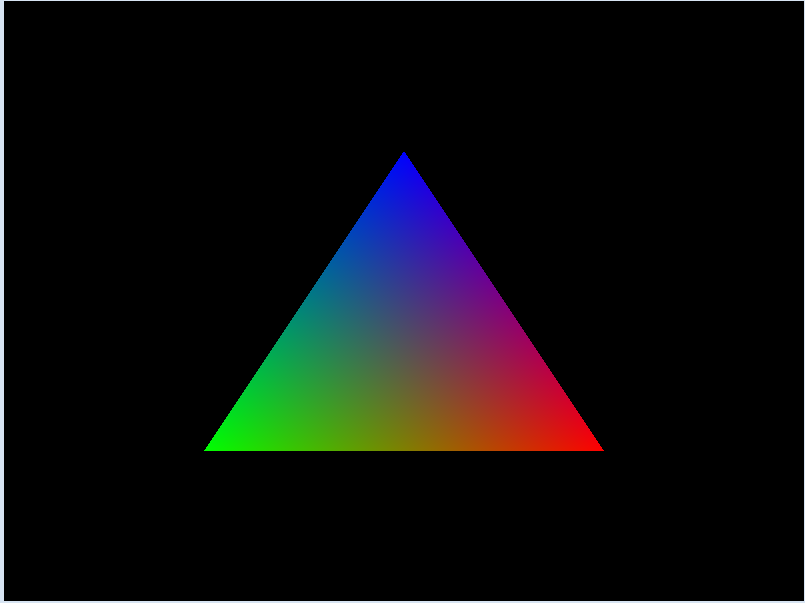
\includegraphics[height=1.75in]{triangle_5.PNG}




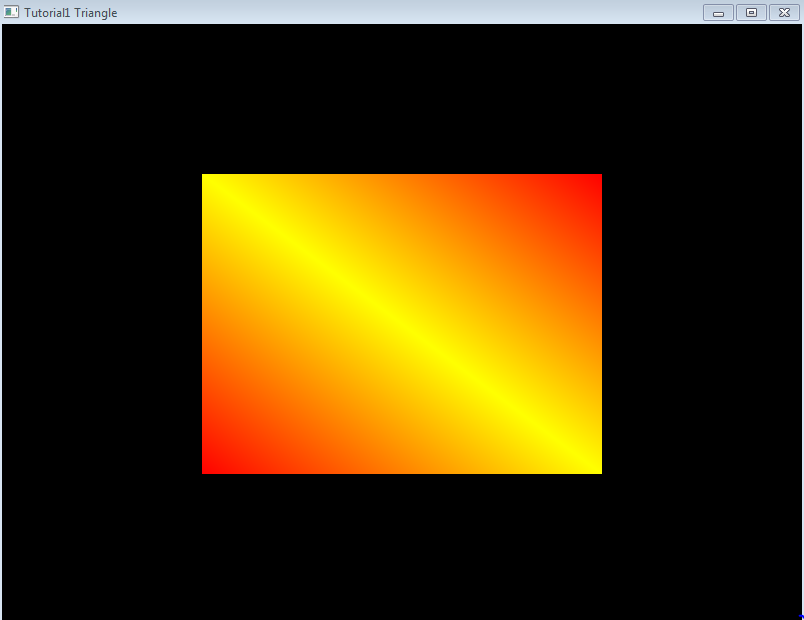
\includegraphics[height=1.75in]{square.PNG}


\pagebreak

	
\end{document}